\documentclass{article}
\usepackage{booktabs}
\usepackage{amsmath}
\usepackage{amssymb}
\usepackage[noend]{algorithmic}
\usepackage[nothing]{algorithm}
\usepackage{tikz}
\usepackage{latexsym}
\usepackage{float}
\usepackage{mathrsfs}
\providecommand{\e}[1]{\ensuremath{\times 10^{#1}}}
\renewcommand{\thealgorithm}{}
\usetikzlibrary{arrows}
\title{CS 522: Data Structures and Algorithms II \\ Homework 2}
\author{Dustin Ingram}
\begin{document}
\maketitle
\begin{enumerate}
    \item \textbf{Solution:}
    We split the edge $(u,v)$:
    \begin{figure}[H]
    \centering
    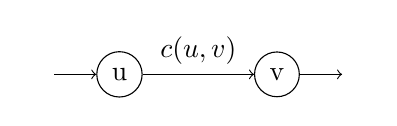
\begin{tikzpicture}[]
    \node [circle,draw] (1){u};
    \node [circle,draw,right of=1, xshift=1cm] (2){v};
    \node [circle,left of=1] (l){};
    \node [circle,right of=2] (r){};
    \path [draw, ->] (l)--(1);
    \path [draw, ->] (2)--(r);
    \path [draw, ->] (1)--(2) node [midway, above] {$c(u,v)$};
    \end{tikzpicture}
    \end{figure}
    Into edges $(u,x)$ and $(x,v)$:
    \begin{figure}[H]
    \centering
    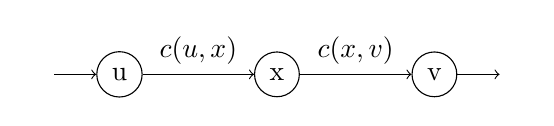
\begin{tikzpicture}[]
    \node [circle,draw] (1){u};
    \node [circle,draw,right of=1, xshift=1cm] (3){x};
    \node [circle,draw,right of=3, xshift=1cm] (2){v};
    \node [circle,left of=1] (l){};
    \node [circle,right of=2] (r){};
    \path [draw, ->] (l)--(1);
    \path [draw, ->] (2)--(r);
    \path [draw, ->] (1)--(3) node [midway, above] {$c(u,x)$};
    \path [draw, ->] (3)--(2) node [midway, above] {$c(x,v)$};
    \end{tikzpicture}
    \end{figure}
    Such that:
    $$ c(u,x) = c(x,v) = c(u,v) $$
    Since the amount of potential flow into and out of $x$ is the same, one can
    show that it is equivalent with the edge $(u,v)$. There are three cases to
    consider:
    \begin{enumerate}
        \item \textbf{$f(s,u) = 0$}: If there is no flow into $u$, there will be
        no flow between $u$ and $x$, and between $x$ and $v$, and the maximum
        flow in $G'$ remains the same.
        \item \textbf{$f(s,u) < c(u,v)$}: If the flow to $u$ is less than the
        potential maximum flow on $(u,x)$ and $(x,v)$, since there is no other
        source of flow for the path, the maximum flow in $G'$ remains the same.
        \item \textbf{$f(s,u) = c(u,v)$}: If the flow to $u$ is equivalent to
        the potential maximum flow of $(u,v)$, and thus $(u,x)$ and $(x,v)$, the
        flows will also be maximized across these edges and the maximum flow in
        $G'$ remains the same.
    \end{enumerate}
    Essentially, any consecutive sets of edges which constitute a single path,
    which do not share any vertex with any other edges, and which have the same
    maximum flow can be simplified into a single edge and the maximum flow of
    the graph will remain the same.

    \item \textbf{Solution:}
    We extend the flow properties and definitions as follows:
    \begin{enumerate}
        \item \textbf{Capacity constraint:} Does not change, edges still cannot
        exceed their maximum potential flow.
        \item \textbf{Flow conservation:} This property does not change, and is
        still true for all $u \in V - {s, t}$ (including super-sources and
        super-sinks).
        \item \textbf{Flow value:} In the original graph, the flow value is
        defined as:
        $$ f = \displaystyle\sum_{v\in V} f(s,v) $$
        The flow from the super-source $s_{s}$ to the regular sources $S \subset
        V$, and from the regular sinks $T \subset V$ to the super-sink $t_{s}$,
        is the same as the flow across the graph. Therefore:
        $$ f = \displaystyle\sum_{v\in V} f(s,v) = \displaystyle\sum_{s\in S}
        f(s_{s},s) = \displaystyle\sum_{t\in T} f(t,t_{s}) $$
        Thus:
        $$ f = \displaystyle\sum_{v\in V} f(s,v) = \displaystyle\sum_{v\in V'}
        f(s_{s}, t_{s}) $$
    \end{enumerate}
    \item \textbf{Solution:}
    If there is a vertex $u$ on the graph $G$ such that there is no path $s
    \leadsto u \leadsto t$, the maximum flow of $G$ must have $f(u,v) = f(v,u) =
    0$ for all vertices $v\in V$. If there is not a path $s \leadsto u \leadsto
    t$, this means that for any path $s \leadsto v \leadsto u$, there is no
    path $s \leadsto v \leadsto u \leadsto t$. Thus any flow along this path
    would not arrive at the sink $t$, and thus:

    $$ \displaystyle\sum_{v\in V} f(s,v) \neq \displaystyle\sum_{v\in V} f(v,t)
    $$

    Specifically because:
    $$ f(s,u) \neq f(u,t) $$
    Where $u$ is the violating vertex. The only case where this would not
    violate this maximum-flow property is that in which:

    $$ f(u,v) = f(v,u) = 0, v\in V $$

    Which makes the flow $f(s,v)$ equivalent to the (non-existent) flow
    $f(v,t)$, and satisfies:

    $$ \displaystyle\sum_{v\in V} f(s,v) = \displaystyle\sum_{v\in V} f(v,t) $$

    \item \textbf{Solution:}
    The graph $G$ of the flow network with multiple sources $s_{i}$ and sinks
    $t_{j}$ is as follows:

    \begin{figure}[H]
    \centering
    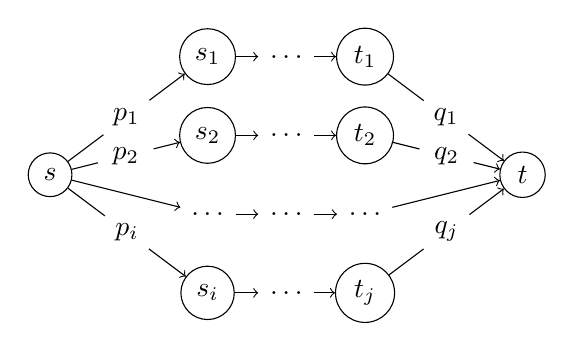
\begin{tikzpicture}[every node/.style={circle}
    ]
    \node[draw] (0) {$s$};
    \node[draw, right of=0, xshift=1cm, yshift=1.5cm] (1){$s_{1}$};
    \node[draw, below of=1] (2){$s_{2}$};
    \node[below of=2] (3){$\ldots$};
    \node[draw, below of=3] (4){$s_{i}$};
    \path[draw, ->] (0)--(1) node[midway,circle,fill=white] {$p_{1}$};
    \path[draw, ->] (0)--(2) node[midway,circle,fill=white] {$p_{2}$};
    \path[draw, ->] (0)--(3);
    \path[draw, ->] (0)--(4) node[midway,circle,fill=white] {$p_{i}$};
    \node[right of=1] (1m){$\ldots$};
    \node[right of=2] (2m){$\ldots$};
    \node[right of=3] (3m){$\ldots$};
    \node[right of=4] (4m){$\ldots$};
    \path[draw, ->] (1)--(1m);
    \path[draw, ->] (2)--(2m);
    \path[draw, ->] (3)--(3m);
    \path[draw, ->] (4)--(4m);
    \node[draw, right of=1m] (1j){$t_{1}$};
    \node[draw, right of=2m] (2j){$t_{2}$};
    \node[right of=3m] (3j){$\ldots$};
    \node[draw, right of=4m] (4j){$t_{j}$};
    \path[draw, ->] (1m)--(1j);
    \path[draw, ->] (2m)--(2j);
    \path[draw, ->] (3m)--(3j);
    \path[draw, ->] (4m)--(4j);
    \node[draw, right of=2j, xshift=1cm, yshift=-.5cm] (t) {$t$};
    \path[draw, ->] (1j)--(t) node[midway,circle,fill=white] {$q_{1}$};
    \path[draw, ->] (2j)--(t) node[midway,circle,fill=white] {$q_{2}$};
    \path[draw, ->] (3j)--(t);
    \path[draw, ->] (4j)--(t) node[midway,circle,fill=white] {$q_{j}$};
    \end{tikzpicture}
    \end{figure}

    For every source, there is a unit of flow $p_{i}$ which is delivered to the
    graph, and for every sink, there is a unit of flow $q_{j}$ which leaves the
    graph.  Since these values are guaranteed for each source or sink vertex, we
    can reduce the problem of finding a flow $f$ in $G$ to a single-source,
    single-sink problem by converting all $s_{i}$ and $t_{j}$ to regular
    vertices on the graph, and converting the edges from $s \rightarrow s_{i}$ to
    regular edges, such that $c(s, s_{i}) = p_{i}$ and similarly the edges from
    $t_{j} \rightarrow {t}$ to edges such that $c(t_{j}, t) = q_{j}$.

    \item \textbf{Solution:}
    Using the \textsc{Max-Flow} algorithm, we can determine the edge
    connectivity of the undirected graph $G$ with vertices $V$ and edges $E$ as
    follows. First, we select any two vertices $s,t \in V$ as the source and
    sink. Then, for every undirected edge $(u,v)\in E$, we create the directed
    edges $(u,v)$ and $(v,u)$ and make their capacity such that $c(u,v) = c(v,u)
    = 1$. We then use $|V|$ applications of the \textsc{Max-Flow} algorithm to
    determine the maximum total flow of the graph, which is equivalent to the
    edge connectivity of the original undirected graph $G$.

    \item \textbf{Solution:}
    An edge entering the source on a flow network $G$ represents a cycle between
    the source $s$ and any number of vertices $v \in V$. The figures below provide
    an example for $G$:

    \begin{figure}[H]
    \centering
    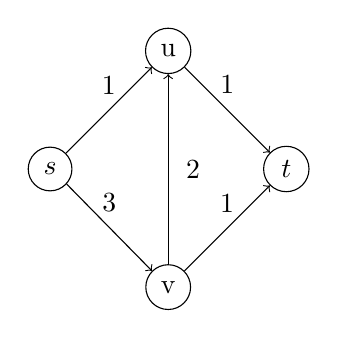
\begin{tikzpicture}[every node/.style={circle, minimum size=.55cm}
    ]
    \node[draw] (s) {$s$};
    \node[draw, right of=s, xshift=2cm] (t) {$t$};
    \node[draw, right of=s, xshift=.5cm, yshift=1.5cm] (1){u};
    \node[draw, right of=s, xshift=.5cm, yshift=-1.5cm] (2){v};
    \path[draw, ->] (s)--(1) node[midway,above,circle,minimum size=0cm] {1};
    \path[draw, ->] (s)--(2) node[midway,above,circle,minimum size=0cm] {3};
    \path[draw, ->] (2)--(1) node[midway,right,circle,minimum size=0cm] {2};
    \path[draw, ->] (2)--(t) node[midway,above,circle,minimum size=0cm] {1};
    \path[draw, ->] (1)--(t) node[midway,above,circle,minimum size=0cm] {1};
    \end{tikzpicture}
    \hspace{.4cm}
    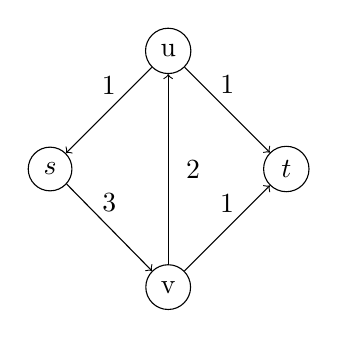
\begin{tikzpicture}[every node/.style={circle, minimum size=.55cm}
    ]
    \node[draw] (s) {$s$};
    \node[draw, right of=s, xshift=2cm] (t) {$t$};
    \node[draw, right of=s, xshift=.5cm, yshift=1.5cm] (1){u};
    \node[draw, right of=s, xshift=.5cm, yshift=-1.5cm] (2){v};
    \path[draw, ->] (1) -- node[midway,above,circle,minimum size=0cm] {1} (s);
    \path[draw, ->] (s) -- node[midway,above,circle,minimum size=0cm] {3} (2);
    \path[draw, ->] (2) -- node[midway,right,circle,minimum size=0cm] {2} (1);
    \path[draw, ->] (2) -- node[midway,above,circle,minimum size=0cm] {1} (t);
    \path[draw, ->] (1) -- node[midway,above,circle,minimum size=0cm] {1} (t);
    \end{tikzpicture}
    \hspace{.4cm}
    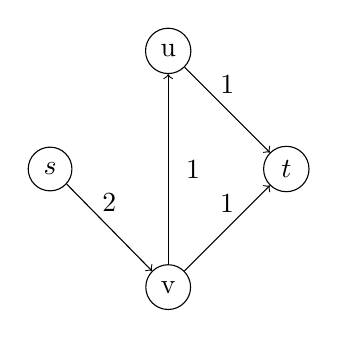
\begin{tikzpicture}[every node/.style={circle, minimum size=.55cm}
    ]
    \node[draw] (s) {$s$};
    \node[draw, right of=s, xshift=2cm] (t) {$t$};
    \node[draw, right of=s, xshift=.5cm, yshift=1.5cm] (1){u};
    \node[draw, right of=s, xshift=.5cm, yshift=-1.5cm] (2){v};
    \path[draw, ->] (s) -- node[midway,above,circle,minimum size=0cm] {2} (2);
    \path[draw, ->] (2) -- node[midway,right,circle,minimum size=0cm] {1} (1);
    \path[draw, ->] (2) -- node[midway,above,circle,minimum size=0cm] {1} (t);
    \path[draw, ->] (1) -- node[midway,above,circle,minimum size=0cm] {1} (t);
    \end{tikzpicture}
    \end{figure}

    Here, the first graph is $G$ with all of it's original edges and their
    maximum capacities. The second graph is an example flow $f$ of $G$ in which
    the max flow $f=2$, and $f'(v,s)=1$. The third graph is another flow $f'$
    with the cycle removed, such that $f'=2$ is still true, however $f'(v,s)=0$.

    A cycle $s\leadsto s$ represents ``wasted'' flow in the flow network of $G$,
    as the flow is not entering the sink $t$ but instead returning to the vertex
    $s$. An algorithm to compute $f'$ from $f$ removes this cycle:

    \begin{enumerate}
        \item Identify a path $p_{cycle}$ in $G$ such that $s\leadsto s$;
        \item Determine the minimum capacity $c_{cycle}$ of all $e \in p_{cycle}$;
        \item For every $e \in p_{cycle}$, reduce the flow of $e$ by
        $c_{cycle}$.
    \end{enumerate}

    Since we are removing the entire capacity from at least one edge in the
    cycle, we are breaking the cycle and eliminating the ``wasted'' flow. Since
    we are traversing at most $E$ edges, the complexity of this algorithm would
    be $O(E)$.

    In the figures above, the path of the cycle is $p_{cycle} = s \rightarrow u
    \rightarrow v$, and the maximum capacity of the cycle is $c_{cycle} = 1$.

    \item \textbf{Solution:}
    \begin{enumerate}
        \item In a flow network in which vertices \emph{and} edges have
        capacities, it is trivial to reduce the network to an ordinary maximum
        flow problem on a flow network of a comparable size. Each vertex which
        has a capacity can be converted into a pair of vertices with a single
        edge between them with a capacity equal to the capacity of that vertex.
        Each edge entering the original vertex would enter one node, and each
        edge exiting the original vertex would exit the second.  This would
        result in an increase of vertices and edges from $G(V, E)$ to at most
        $G(V+V, E+V)$.
        \item To solve the escape problem, we can reduce it to a form of a
        flow network and solve it via \textsc{Max-Flow}. To convert the
        undirected $n\times n$ escape grid into a flow network, we must take the
        following into consideration:
        \begin{enumerate}
            \item Paths may not pass through unoccupied vertices more than once;
            \item Paths may not pass through edges more than once;
            \item Every occupied vertex must be able to escape;
            \item Every unoccupied border vertex is a goal destination.
        \end{enumerate}
        To satisfy these restraints, we modify the grid as follows:
        \begin{enumerate}
            \item Every unoccupied vertex is given a capacity of $c = 1$, and
            reduced as described in (a);
            \item Every undirected edge is given has a bi-directional capacity $c
            = 1$;
            \item A new vertex, $s$ is added to the graph, and given an edge to
            every occupied vertex in the grid for which $c = \infty$, which will
            be the source;
            \item A new vertex, $t$ is added to the graph, and given an edge to
            every $4n-4$ border vertices for which $c = \infty$, which will be
            the sink.
        \end{enumerate}
        One can then use \textsc{Max-Flow} to find the maximum flow through the
        new graph. A graph which is fully ``escapable'' will have a maximum flow
        equal to the number of starting points within the graph.

        \textbf{Complexity:} In the original grid, there were $n^{2}$ nodes and
        $2n^{2}-2n$ edges. After converting the grid to a simple flow network,
        we have increased the vertices by at most $n^2$ (by splitting capacitive
        vertices) and the edges by $n^{2}$ (by adding edges to the source) plus
        $4n-4$ (by adding edges to the border vertices) plus an additional
        $2n^2-2n$ (by splitting all undirected edges). Thus, the number of
        vertices and edges in the flow network are:
        \begin{align*}
            V &= (n^2) + (n^2) = 2n^2 = O(n^2) \\
            E &= (2n^2-2n) + (n^2) + (4n-4) + (2n^2-2n) = 5n^2 - 4 = O(n^2)
        \end{align*}
        Thus if we were to use an algorithm such as the \textsc{Ford-Fulkerson}
        algorithm, the total runtime would be:

        $$ O(E|f^*|) = O(n^2\cdot 4n-4) = O(n^3) $$

        Where $f^*=4n-4$ is the maximum flow, which is limited by the number of
        possible escape vertices on the border of the grid.
    \end{enumerate}

    \item \textbf{Solution:}
    \begin{enumerate}
        \item We turn $G$ into a bipartite graph $G'=(V',E')$ such that:
        \begin{align*}
            V' &= \{x_0, x_1, \ldots, x_n\} \cup \{y_0, y_1, \ldots, y_n\} \\
            E' &= \{(x_0, x_i):i\in V\}\cup \{(y_i,y_0):i\in V\}\cup
            \{(x_i,y_j):(i,j)\in E\}
        \end{align*}
        We then assign a capacity $c = 1$ to every edge in the graph, and use
        \textsc{Max-Flow} to determine the maximum flow of $G'$, using $x_0$ as
        the source and $y_0$ as the sink. The edges which cross the bipartite
        graph (that is edges of the form $(x_i, y_j)$) correspond to edges in
        the optimal path cover of $G$.
        \item The algorithm will only work on directed acyclic graphs. This is
        because the algorithm will complete every cycle in the resulting graph
        to increase the flow, even though cycles do not exist in an optimal path
        covering (they have one more edge than is necessary).
    \end{enumerate}
\end{enumerate}
\end{document}
